%!TEX root = paper.tex
\section{Overview}
Before formally defining the problem tackled by \name and the algorithms, 
we present an overview of \name using an end-to-end
example. Consider the hierarchical network in \Cref{fig:example} which
is split into three OSPF domains, and these domains communicate
using BGP. Host A talks to hosts B and C with the following policies:
traffic to B must go through a firewall at router $R_3$, traffic to C 
goes through an IDS at $R_5$ and traffic 
to B and C do not share any links (We discuss the policies supported in
detail in \Cref{sec:policy}). \name 
synthesizes OSPF and BGP router configurations satisfying the 
policies. Illustrating our two-phase approach (\Cref{fig:architecture}), 
\name first uses \genesis~\cite{genesis}, a policy-enforcement framework for SDNs 
to find policy-compliant paths (indicated by the blue and
red paths). Note that there exists multiple solutions for the given
policies, we show how the control plane is synthesized using one of the solutions:
\begin{figure}
	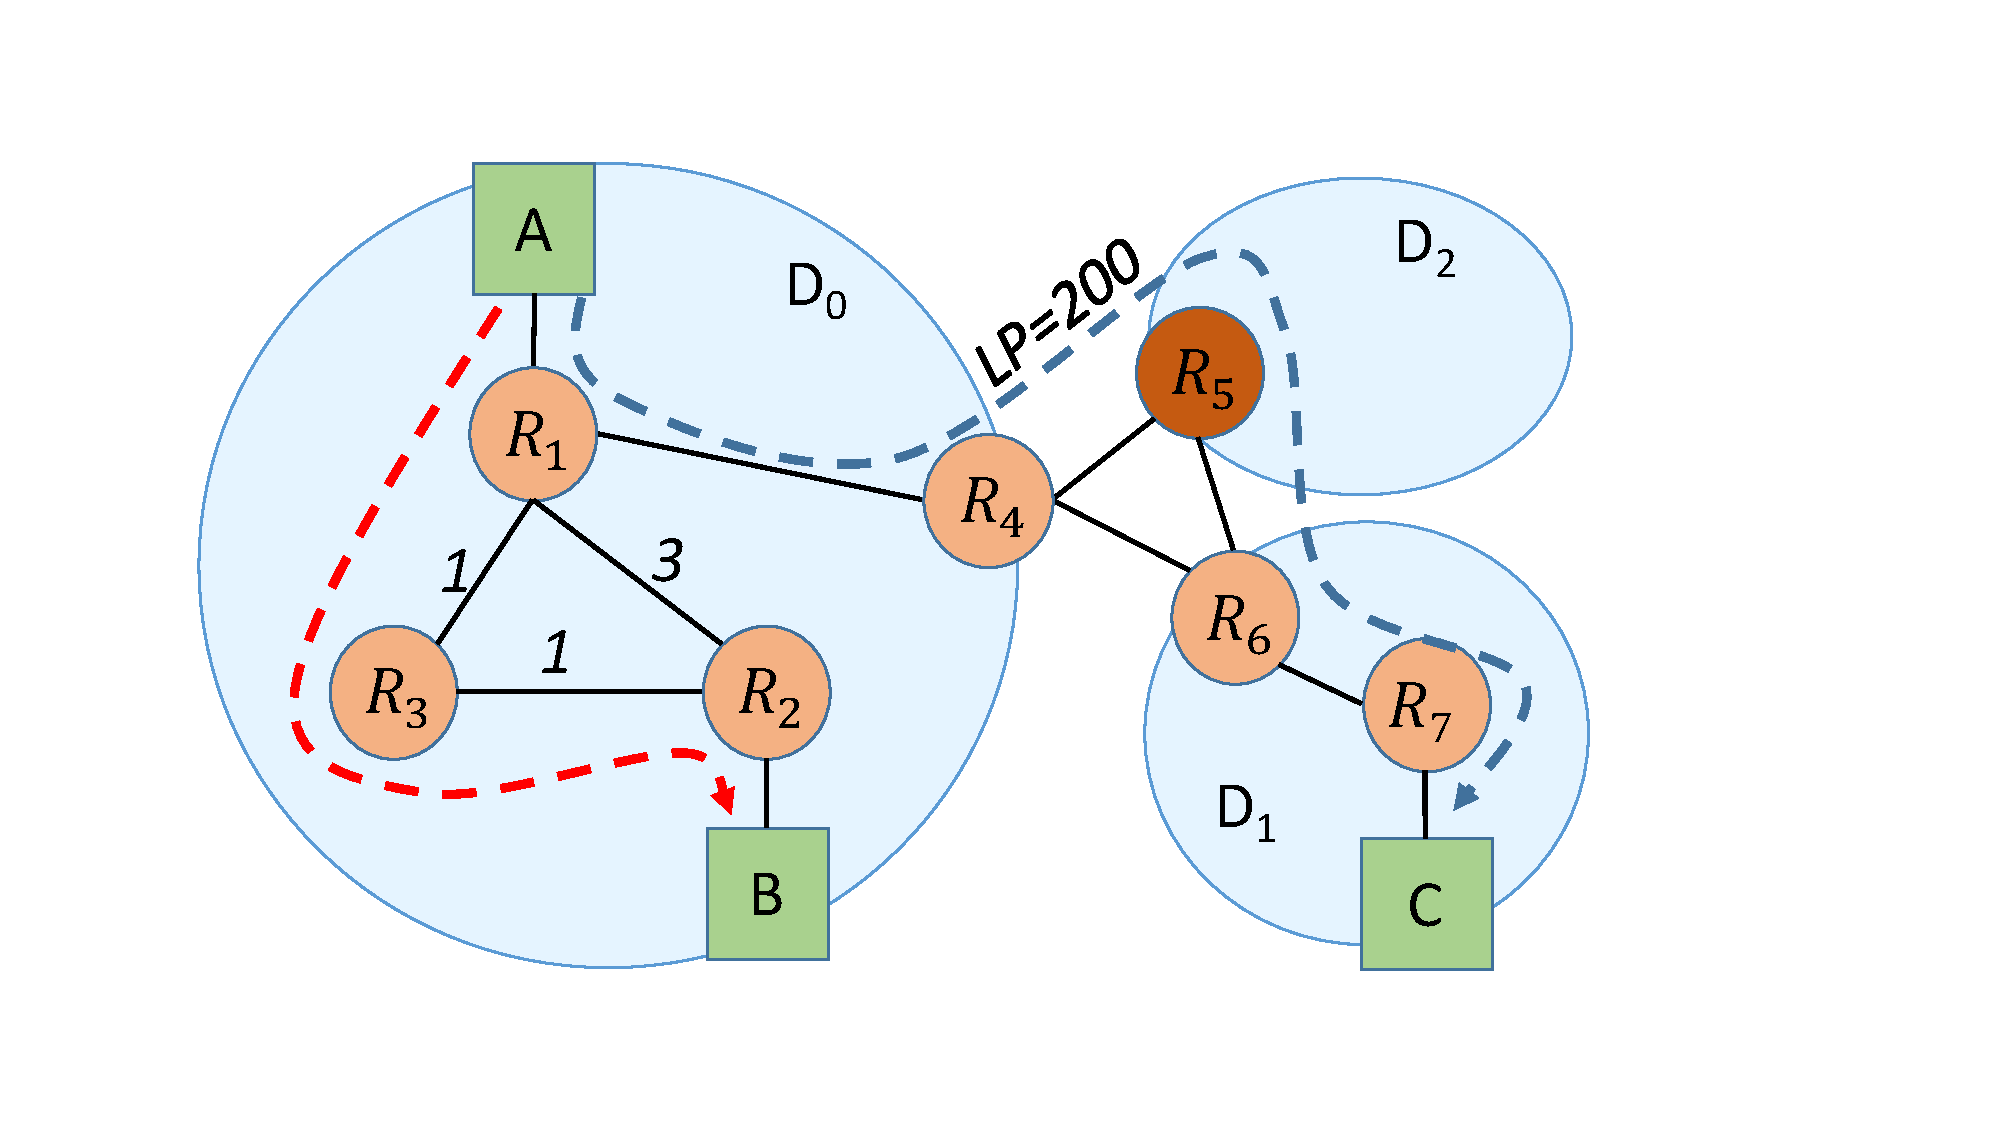
\includegraphics[width=0.5\columnwidth]{figures/example.pdf}
	\caption{Example demonstrating the two-phase synthesis approach. 
	Genesis produces policy-compliant paths (red and blue), 
	which are used as input by \name to
	synthesize the OSPF and BGP configurations.}
	\label{fig:example}
\end{figure}

\begin{itemize}
	\item
For traffic $A \rightarrow B$, the path is entirely inside
a single OSPF domain, so \name has to find OSPF weights 
such that the shortest path is $R_1 \rightarrow R_3 \rightarrow 
R_2$. From the OSPF weights shown in \Cref{fig:example}, 
we can see that the weight of path $R_1 
\rightarrow R_3 \rightarrow R_2$ (2) is smaller than that of path
$R_1 \rightarrow R_2$ (5). 
 	\item For traffic $A \rightarrow C$, the path traverses through 
 	multiple domains, so \name configures BGP such that 
 	routing across domains follows the Genesis path. In this case, 
 	we need traffic to go through a longer path in terms of AS path
 	length; \name sets $R_4$'s BGP local preference for route C
 	from $R_5$ to a higher value (200), so that $R_5$ is 
 	preferred over $R_6$. 
 	\item \name can find better control planes in terms of how 
 	the network is split into domains. In this case,  
 	\name will suggest moving $R_5$ to domain $D_1$. 
 	This simplifies $R_4$'s BGP configuration as the local preference 
 	entry for C is not required. 
 	\item With a backup firewall at $R_8$, 
 	\name automatically synthesizes resilient OSPF configurations
          for $D_0$ such that if either $R_1-R_3$ or $R_3-R_2$ link
          fails, traffic to B goes through the firewall at $R_8$.
\end{itemize}
\name is fundamentally different from state-of-art approaches for policy enforcement
in legacy networks: Propane~\cite{propane} generates BGP configurations
from peering and path requirements, while Fibbing~\cite{fibbing} uses fake
advertisements to centrally control OSPF routing. SyNET~\cite{synet} targets
BGP and OSPF configuration synthesis, however, it does not cleanly
tackle domain assignments or provide support for resilience. 
\name has more general policy coverage, supports automatic domain assignment 
(which is manual and difficult today), and can provide fault-tolerant configurations, all in one system.
